\documentclass[class=NCU_thesis, crop=false]{standalone}
\begin{document}

\chapter{背景知識與文獻回顧}
\section{背景知識}

本章節將會介紹本論文所需的背景知識,可以幫助讀者更好地理解本論文提出的論文的概念和出發點,
內容包含:人如何感知彩色影像、大腦皮質的運作、卷積神經網路與以卷積神經網路為基礎的可解釋性深度學習模型。

\subsection{人如何感知彩色影像}

要了解人如何感知色彩我們必須要先了解將彩色影像的這條 Central Visual Pathway 會經過哪些的部位與流程,
根據《 Neuroscience 》 \cite{Purves2004Neuroscience3E}所介紹,
彩色影像在 Central Visual Pathway 會經過的部位總共可以分為三個重要部位:視網膜(Retina)、外側膝狀體(外膝體,Lateral Geniculate Nucleus)、視覺皮層(Visual Cortex),
彩色影像從視網膜進入後會送入外膝體,外膝體在收到兩側眼球的資訊後會將不同的資訊平行傳輸至不同的視覺皮層,視覺皮層則負責對這些資訊進行分層的整合與感知。
詳細的Central Visual Pathway 如\cref{fig:Central_Visual_Pathway}

\begin{figure}[H]
  \centering
  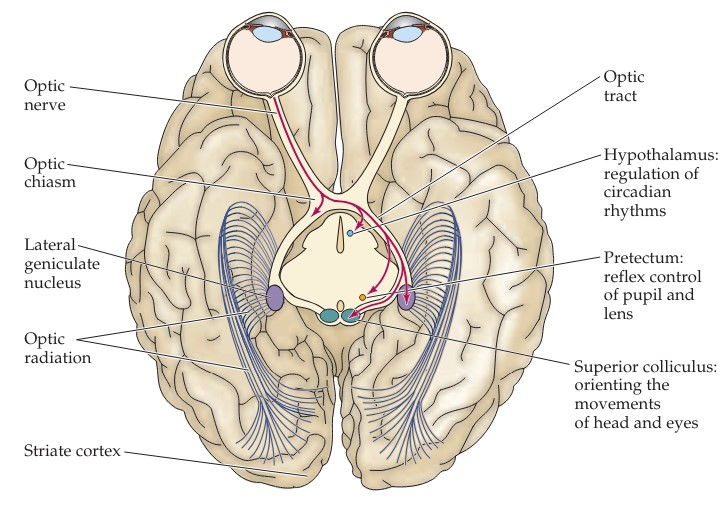
\includegraphics[width=0.7\textwidth]{Visual_Pathway/Central_Visual_Pathway.jpg}
  \caption{詳細視覺路徑圖~\cite{Purves2004Neuroscience3E}}
  \label{fig:Central_Visual_Pathway}
\end{figure}

\subsubsection{視網膜}

外界事物將光反射進入眼睛當中,透過眼珠中的角膜與水晶體等透明的光學介質進行折射最終聚焦於視網膜表面的感光層上形成影像。
在光聚焦於視網膜表層時,視網膜會將光轉換成動作電位並透過視神經傳輸至外膝體,也因此Central Visual Pathway 才會將視網膜視為感知彩色影像的第一個重要部位。

根據《Neuroscience-Exploring the Brain》\cite{bear2016neuroscience}
我們知道視網膜的基礎架構是由五類細胞組成如\cref{fig:RetinaBasic},分別是: 感光細胞、 水平細胞、 無長突細胞、 雙極細胞、 神經節細胞。 感光細胞包含我們常聽到的視錐細胞等負責將輸入的光轉化為動作電位、 雙極細胞負責將會將感光細胞的電位傳送到神經節細胞、
這個傳輸的過程有些則是由水平細胞和無長突細胞協助傳輸,
神經節細胞則負責將最後的資訊傳輸到外膝體之中。

\begin{figure}[H]
  \centering
  \subcaptionbox{
    視網膜基本架構~\cite{bear2016neuroscience}
    \label{fig:RetinaBasic}}
    {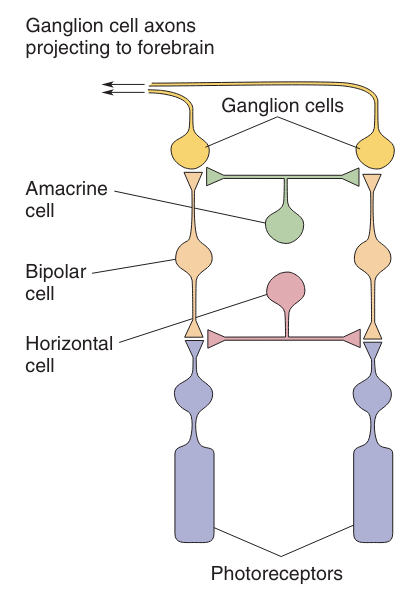
\includegraphics[width=0.5\textwidth]{Visual_Pathway/RetinaBasic.png}
    }
~
  \subcaptionbox{
    視網膜層級架構~\cite{bear2016neuroscience}
    \label{fig:RetinaStructure}
  }
    {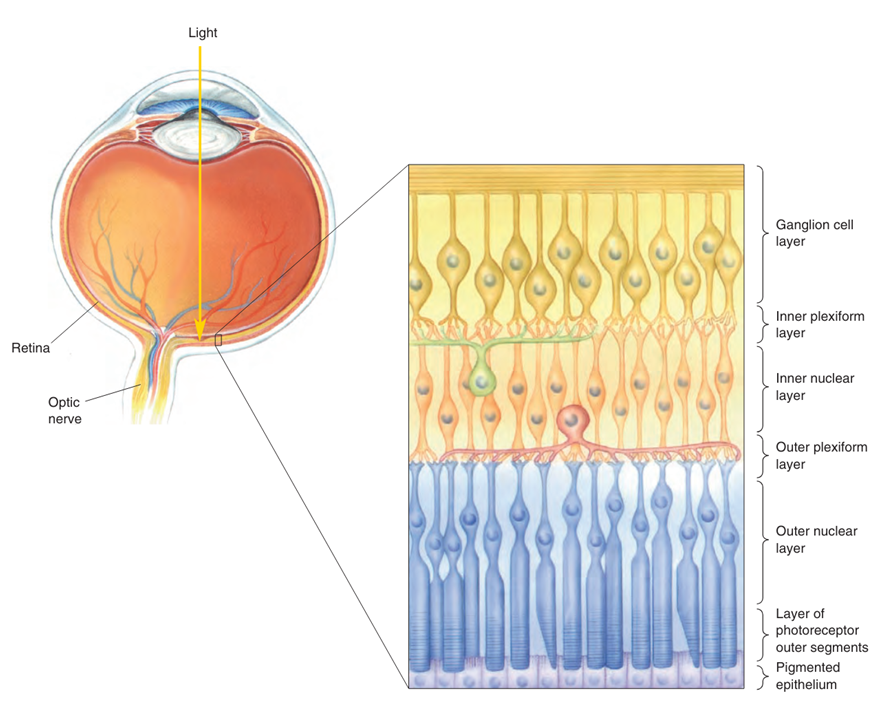
\includegraphics[width=0.9\textwidth]{Visual_Pathway/RetinaStructure.png}
    }
  \caption{視網膜整體架構}
  \label{fig:RetinaTotalStructure}
\end{figure}

上面講的基礎架構只是最基本的情況,事實上視網膜的各類細胞遠比上面要架構要複雜許多,上述的五大類細胞還可以再更細的分為不同功能的變種細胞,由此組成了極度複雜的視網膜層級系統如\cref{fig:RetinaStructure}。
如此複雜的視網膜系統,其功能當然不只負責影像的感知與電位傳輸,事實上
在2013年的\cite{annurev},就已經發現在感光細胞將光轉換為動作電位後會將電位傳輸到層級架構的 Inner Plexiform Layer(IPL)中不同變種的雙極細胞,這些不同變種的雙極細胞對收到的影像資訊進行不同的平行處理,最終輸出影像中不同的方面的要素到神經節細胞,例如: 紅藍綠不同色彩、明暗的變化、影像輪廓等等, 這同時也是本論文在設計彩色影像感知時的核心概念。

\begin{figure}[H]
  \centering
  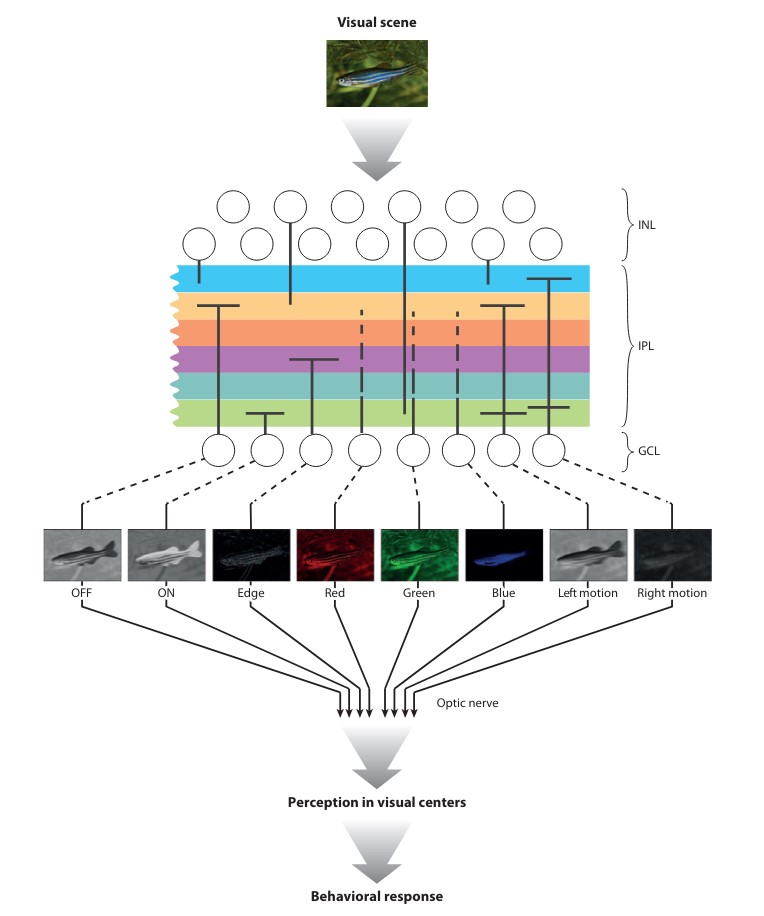
\includegraphics[width=0.7\textwidth]{Visual_Pathway/IPL.jpg}
  \caption{視網膜對影像進行不同的平行處理~\cite{annurev}}
  \label{fig:IPL}
\end{figure}


此外,在Jeff Hawkins的著作\cite{10.5555/993636}和《Principles of Neural Science》\cite{1180370208}中均有提到,
視網膜能接收到的影像資訊不只是上述的空間性資訊,
同時也具有不同時間性的資訊,這代表同樣的影像進入視網膜的型態是會隨時間而改變。
具體而言,眼睛會在每一秒鐘快速移動視線的焦點三到四次(如\cref{fig:Saccade}),
但人類的認知上不會有所感覺,這個行為被稱為 「 眼球跳動 」(Saccade)。
眼球跳動使得同一個影像產生時間上的變化,形成時間性的影像資訊。
這個概念也被運用於本論文的空間位置保留機制中的時間遺忘參數上,
使得影像特徵可以呈現時序上的不同。

\begin{figure}[H]
  \centering
  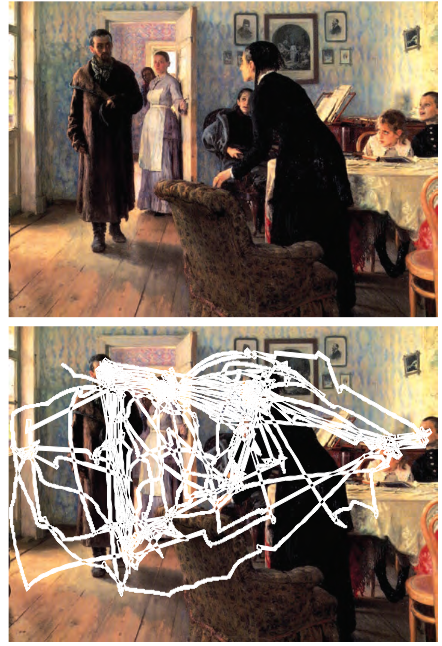
\includegraphics[width=0.7\textwidth]{Visual_Pathway/Saccade.png}
  \caption{眼球跳動示意圖~\cite{annurev}}
  \label{fig:Saccade}
\end{figure}

\subsubsection{外側膝狀體}

外側膝狀體(外膝體)主要負責將視網膜不同的方面資訊(如:色彩、輪廓、運動方向…)傳輸到對應的初級視覺皮質,其中的細胞分層排列,每層分布排列著著不同種類的細胞。
除此之外,外膝體中不同的細胞層也對應著不同視野的半個視網膜形成如 \cref{fig:LGN_Relation}
的對應關係,這也表示視網膜中相鄰區域的同種類的影像資訊在外膝體中很可能在同一個細胞層,
這個性質也保證了外膝體在資訊傳輸的過程可以保留資訊的空間位置資訊。
由於視覺皮層會將影像資訊從初級到高級逐漸進行資訊整合和學習,
因此外膝體的存在可以協助視覺皮層將不同的影像資訊傳輸到對應的視覺皮質層,
這對視覺皮質能夠進行平行處理與整合起到至關重要的作用。

\begin{figure}[H]
  \centering
  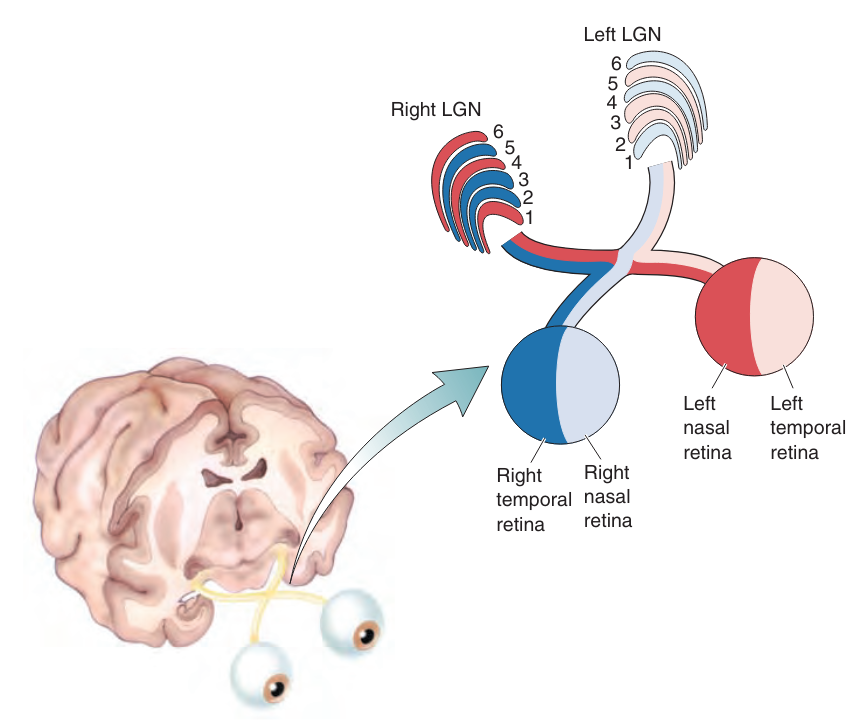
\includegraphics[width=0.7\textwidth]{Visual_Pathway/LGN_relation.png}
  \caption{視網膜與外膝體的對應關係~\cite{bear2016neuroscience}}
  \label{fig:LGN_Relation}
\end{figure}
\pagebreak

\subsubsection{視覺皮層}
皮層可以說是大腦最重要的地方,高級認知功能例如:記憶、思考、感覺等均在此發生。
根據\cite{1180370208}中的說明,人類的大腦中皮質以分層結構存在的,
而視覺皮層又可以分為初級視覺皮層(Primary visual cortex, V1)和紋外皮層(V2、V4、MT層)這四層。
初級視覺皮層負責接收LGN傳輸來的資訊並開始處理顏色、方向、輪廓等視覺資訊,
其餘皮層則負責整合和傳遞資訊給下面的皮層,因此隨著皮層的深入,所得到的視覺資訊也會越來越完整。

\cite{1180370208}提出一種影像資訊處理架構,
示意圖如\cref{fig:ParallelProcess},
其將皮質中的資訊傳輸路徑分成兩類,Ventral Pathway 和 Dorsal Pathway, 
Ventral Pathway 由 V1、V2、V4 組成負責處理影像的色彩、形狀等資訊,
而Dorsal Pathway 由 V1、V2、MT 組成負責處理影像的運動方向的資訊。
但同時也強調這個分類只是一個大致分類,
實際上不同的視覺特徵資訊(如顏色、運動方向等)在皮層中也會相互聯繫,
也就是存在所謂的側向連結,最終才能形成統一的影像感知。

\begin{figure}[H]
  \centering
  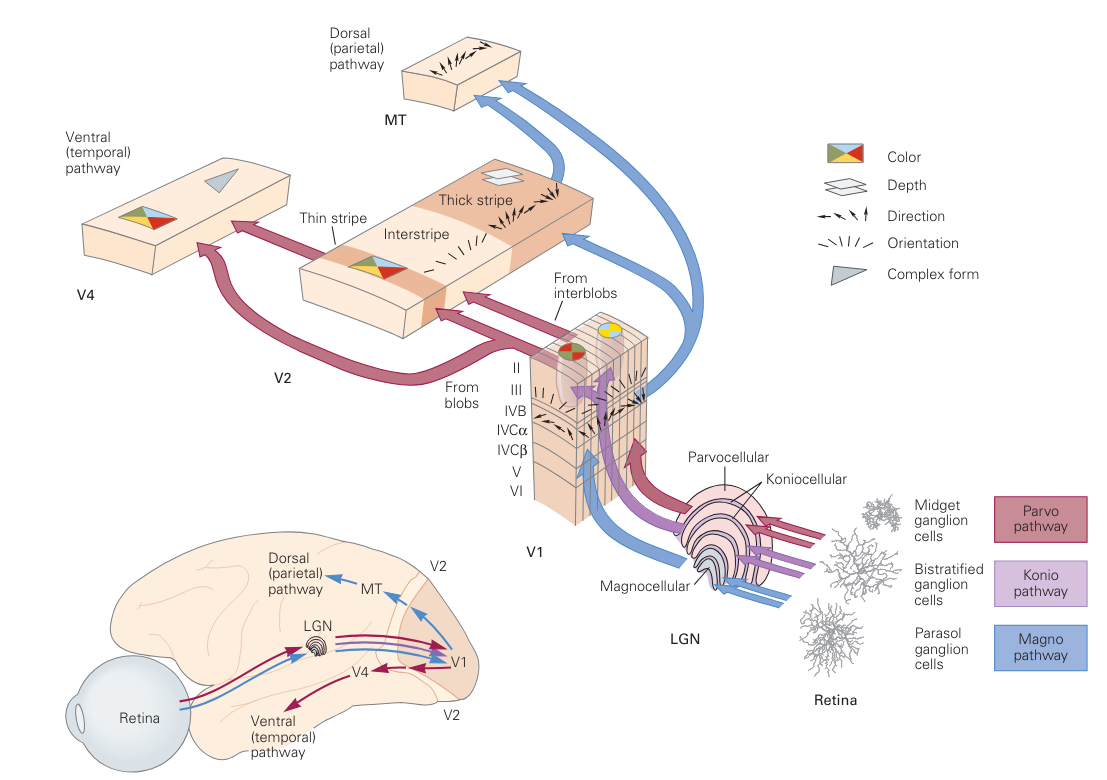
\includegraphics[width=0.8\textwidth]{Visual_Pathway/Parallel_processing_In_contex.png}
  \caption{Visual Pathway的認知過程~\cite{1180370208}}
  \label{fig:ParallelProcess}
\end{figure}

在皮層中,V1 將相同功能的神經束聚在一起形成不同功能的柱狀結構(例如顏色柱、方向柱、線條柱等)
這些柱狀體負責處理各自的視覺資訊並按照固定規則排列成層,
並且將左右眼的柱狀層交錯排列形成一個皮層計算模組(Cortical Computational Module),如\cref{fig:CorticalComputationalModule},重複上百次來覆蓋左右眼看到的所有影像。
這樣設計的目的是希望不管從V1中的任何位置和方向移動都可以漸進的對每塊視野的顏色、輪廓、方向、深度等特徵資訊進行充分的分析。
以上的兩個概念被本論文應用在合併色彩與輪廓特徵與學習綜合特徵中,使我們的模型可以也可以充分學習顏色與輪廓兩個特徵,並隨著層數的深入逐漸組成更完整的影像特徵資訊。

\begin{figure}[H]
  \centering
  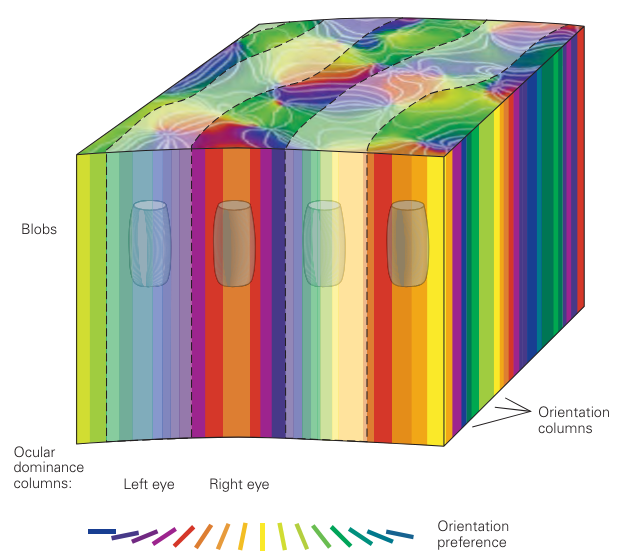
\includegraphics[width=0.7\textwidth]{Visual_Pathway/cortical_computational_module.png}
  \caption{皮層計算模組~\cite{1180370208}}
  \label{fig:CorticalComputationalModule}
\end{figure}
\pagebreak


\subsection{CNN-based Interpretable Model}
CNN-based Interpretable Model(CIM)\cite{YangCNNInterpretable}為 Yang 等人於2023年提出的可解釋性模型,
該模型是模擬大腦視覺皮層的階層架構和影像的時序性關係來解釋深度學習的決策的過程,
目的是希望使模型的決策過程透明化解決黑箱決策的問題。
然而該模型目前只能運用於灰階影像上而無法處理彩色影像的問題,
本論文的目標是基於此模型進行改進,開發出一個更適用於現實彩色影像的新模型。

\subsubsection{模型架構}
該模型採用多層結構,
每層由三個部分組成: 高斯卷積模組、特徵增強模組、空間位置保留合併模組,
整體模型架構如\cref{fig:CIM_arch},
\begin{figure}[H]
  \centering
  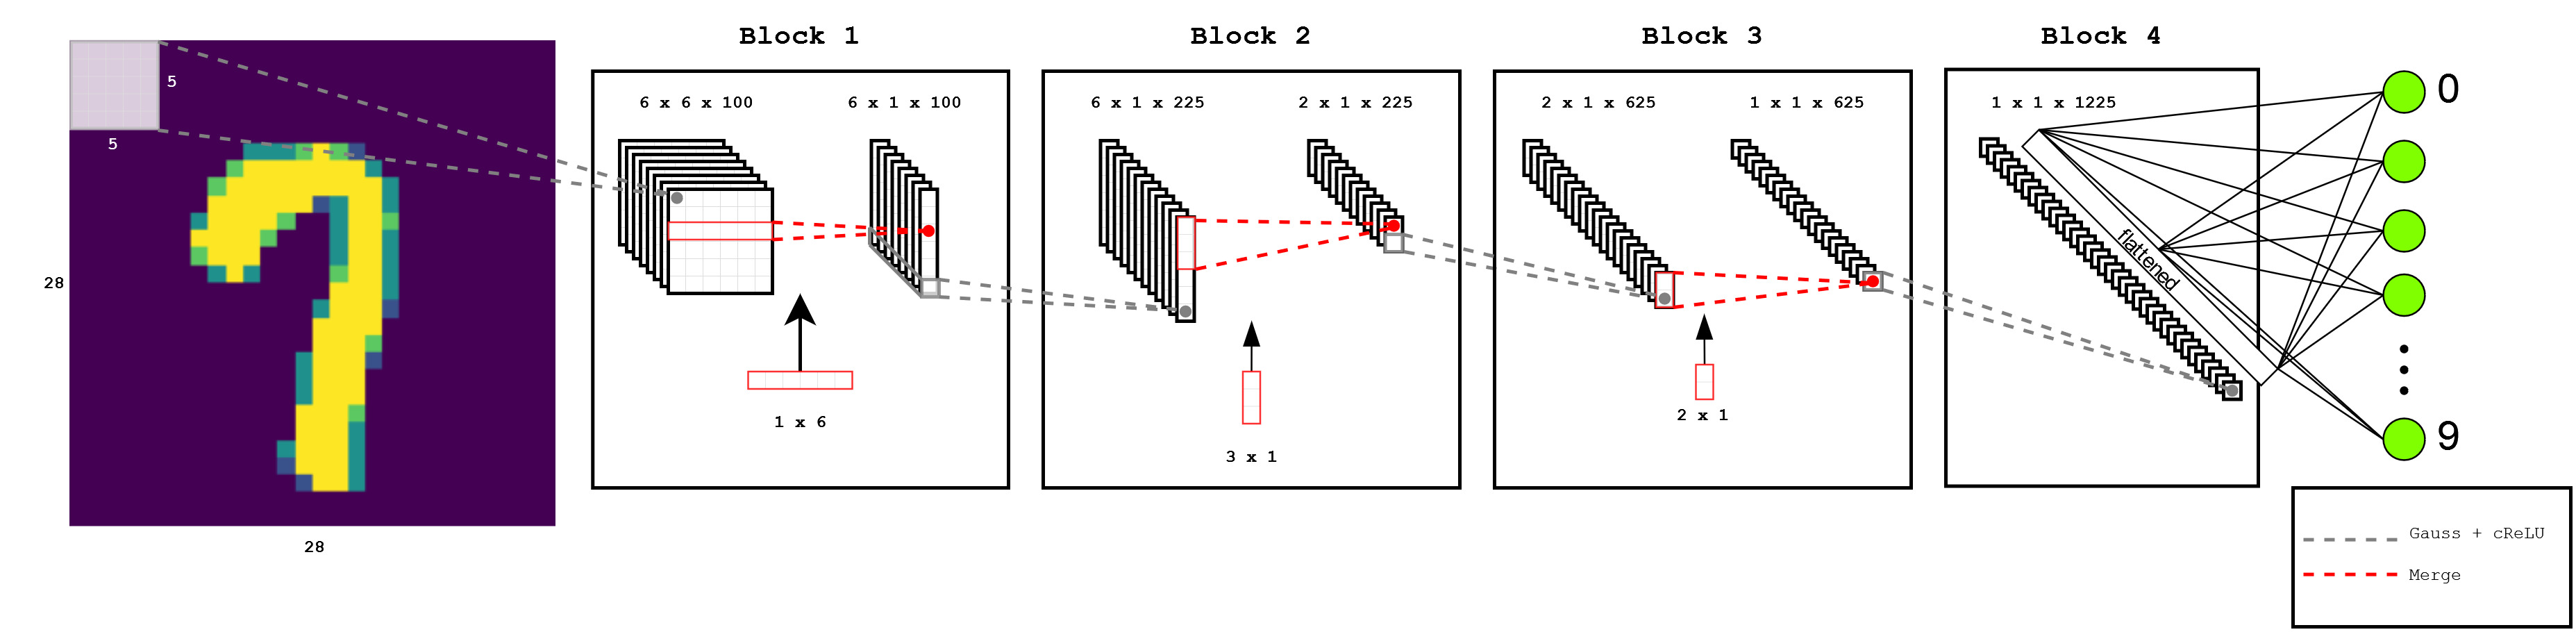
\includegraphics[width=1\textwidth]{CIM/CIM_model_arch.jpg}
  \caption{CIM架構圖~\cite{YangCNNInterpretable}}
  \label{fig:CIM_arch}
\end{figure}


高斯卷積模組使用高斯函數(公式如\cref{eqn:rbf-gaussian-function})取代原始卷積操作中的內積操作來對輸入進行特徵提取,
使得該模組計算的結果具有相似度的意義並且此特性也被運用在後續的可解釋性中。\\
  高斯函數(Gaussian function):\\
  $x$ 為輸入值、$m$ 為中心點、$\sigma$ 為寬度參數
  \begin{equation}
      \label{eqn:rbf-gaussian-function}
      \phi (x) = \exp \left( -\frac{\| x-m \|^2}{2\sigma ^2} \right) 
  \end{equation}

特徵增強模組使用該論文中新提出變形的ReLU函數稱為changed ReLU(簡稱為cReLU)來過濾不重要的特徵使得後續的解釋性可以有更好的發揮。\\
change ReLU的公式如\cref{eq:eq-crelu},$c$為人工取的一個閥值
\begin{equation}
    \label{eq:eq-crelu}
    % f(x) = \max(c, x)
    f(x)= 
    \begin{cases}
        0 & \text{if  $x < c$ }\\
        x & \text{if  $x \geq c$}
    \end{cases}
\end{equation}

空間位置保留合併模組為該論文所提出來的全新機制,
文中他們將一組輸入在經過高斯卷積和特徵增強後產生的輸出稱為$RM$,
而一張影像又擁有多組資訊,從而產生出多張屬於這個影像的$RM$。
使用合併公式\cref{eq:eq-sf}並加入時間遺忘函數(forgetting factor)$\alpha$,來進行合併來模擬特徵資訊在皮層中的時序性特徵資訊與皮層的逐層合併的現象,
從而達到在合併的過程中保留特徵之間的時序關係,
也可讓越後面的層數學習到更完整的特徵資訊。\\
合併公式:\\
$RM_{c}$為合併後的RM,$RM_{k}$為第k張RM,$n$為輸入資訊的數量,$\alpha$為一個可訓練的參
\begin{equation}
    \label{eq:eq-sf}
    RM_{c}=\frac{1}{n} \sum_{k = 0}^{n-1} \alpha^{k} \times RM_{k}  \qquad ,\ where\ n = \textit{H}^{i}_{SF} \times \textit{W}^{i}_{SF}
\end{equation}

\begin{figure}[H]
  \centering
  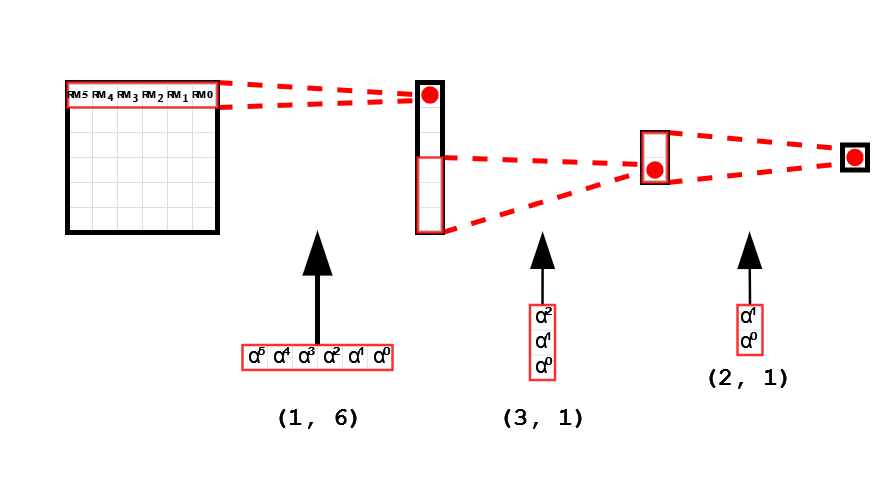
\includegraphics[width=0.7\textwidth]{CIM/CIM_SFM.png}
  \caption{合併方式示意圖~\cite{YangCNNInterpretable}}
  \label{fig:CIM_SFM}
\end{figure}


\subsubsection{可解釋性}
文中將每層的高斯卷積模組的濾波器視為二階矩陣稱為特徵映射圖(Feature Map, $FM$),
一組輸入在每層經過高斯卷積模組和特徵增強模組後的輸出稱為特徵映射響應圖(Response Map, $RM$),
當模型訓練完畢後會讓每個卷積模組中的濾波器對資料集中的所有影像進行反應
並且從所有反應中找到造成最大反應的影像,每個濾波器都會有屬於自己的最大反映影像,
稱為特徵映射圖之對應影像(Corresponding Image, $CI$)
以上的$FM$, $RM$, $CI$ 便是模型提供可解釋性的核心要素,其關係圖如\cref{fig:one-FM2-RM2-CI2-EXAMPLE}

\begin{figure}[H]
    %\captionsetup[subfigure]{labelformat=empty} % 完全隱藏圖號
    \centering
    \subcaptionbox
        {RM$_{0}$之特徵圖
        \label{fig:one-RM2-EXAMPLE}}
        {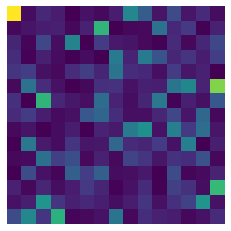
\includegraphics[width=0.33\linewidth]{CIM/fig-one-RM2-EXAMPLE.png}}
    ~
    \subcaptionbox
        {FM$_{0}$之特徵圖
        \label{fig:one-FM2-EXAMPLE}}
        {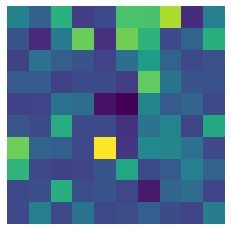
\includegraphics[width=0.33\linewidth]{CIM/fig-one-FM2-EXAMPLE.png}}
    ~
    \subcaptionbox
        {CI$_{0}$之特徵圖
        \label{fig:one-CI2-EXAMPLE}}
        {
\includegraphics[width=0.475\linewidth]{CIM/fig-one-CI2-EXAMPLE.png}}
    \caption{FM-RM-CI\cite{YangCNNInterpretable}}
    \label{fig:one-FM2-RM2-CI2-EXAMPLE}
\end{figure}

在可解釋性的方法上,論文中提出了兩個方法,
第一個方法為特徵圖對應法,
在將一張影像輸入進模型後
第一步視覺化輸入影像中每個區塊在模型中每層的$RM$並找出$RM$中最大反應,
第二步從$RM$最大反應找出造成反應的$FM$,
第三步根據$FM$和$CI$的對應關係,找出該$FM$對應之$CI$,
第四步利用每個區塊的$CI$根據原本的位置組合出輸入影像在模型中被分解的過程
這個方法用於了解模型在經過高斯卷積、特徵增強、空間位置保留合併後所關注的特徵資訊。
範例如\cref{tab:CIM_RMCI_example}

\begin{table}[H]
  \centering
  \begin{tabular}{| c | c | c | c | c |}
    \hline
    原始影像 & RM-CI1 & RM-CI2 & RM-CI3 & RM-CI4 \\
    \hline
    \begin{minipage}[t]{0.18\columnwidth}\centering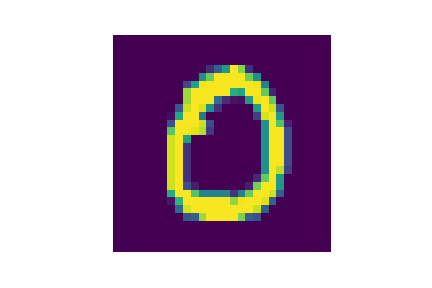
\includegraphics[width=0.9\textwidth]{CIM/mnist-16-0-cmp-input.png}\end{minipage} &
    \begin{minipage}[t]{0.18\columnwidth}\centering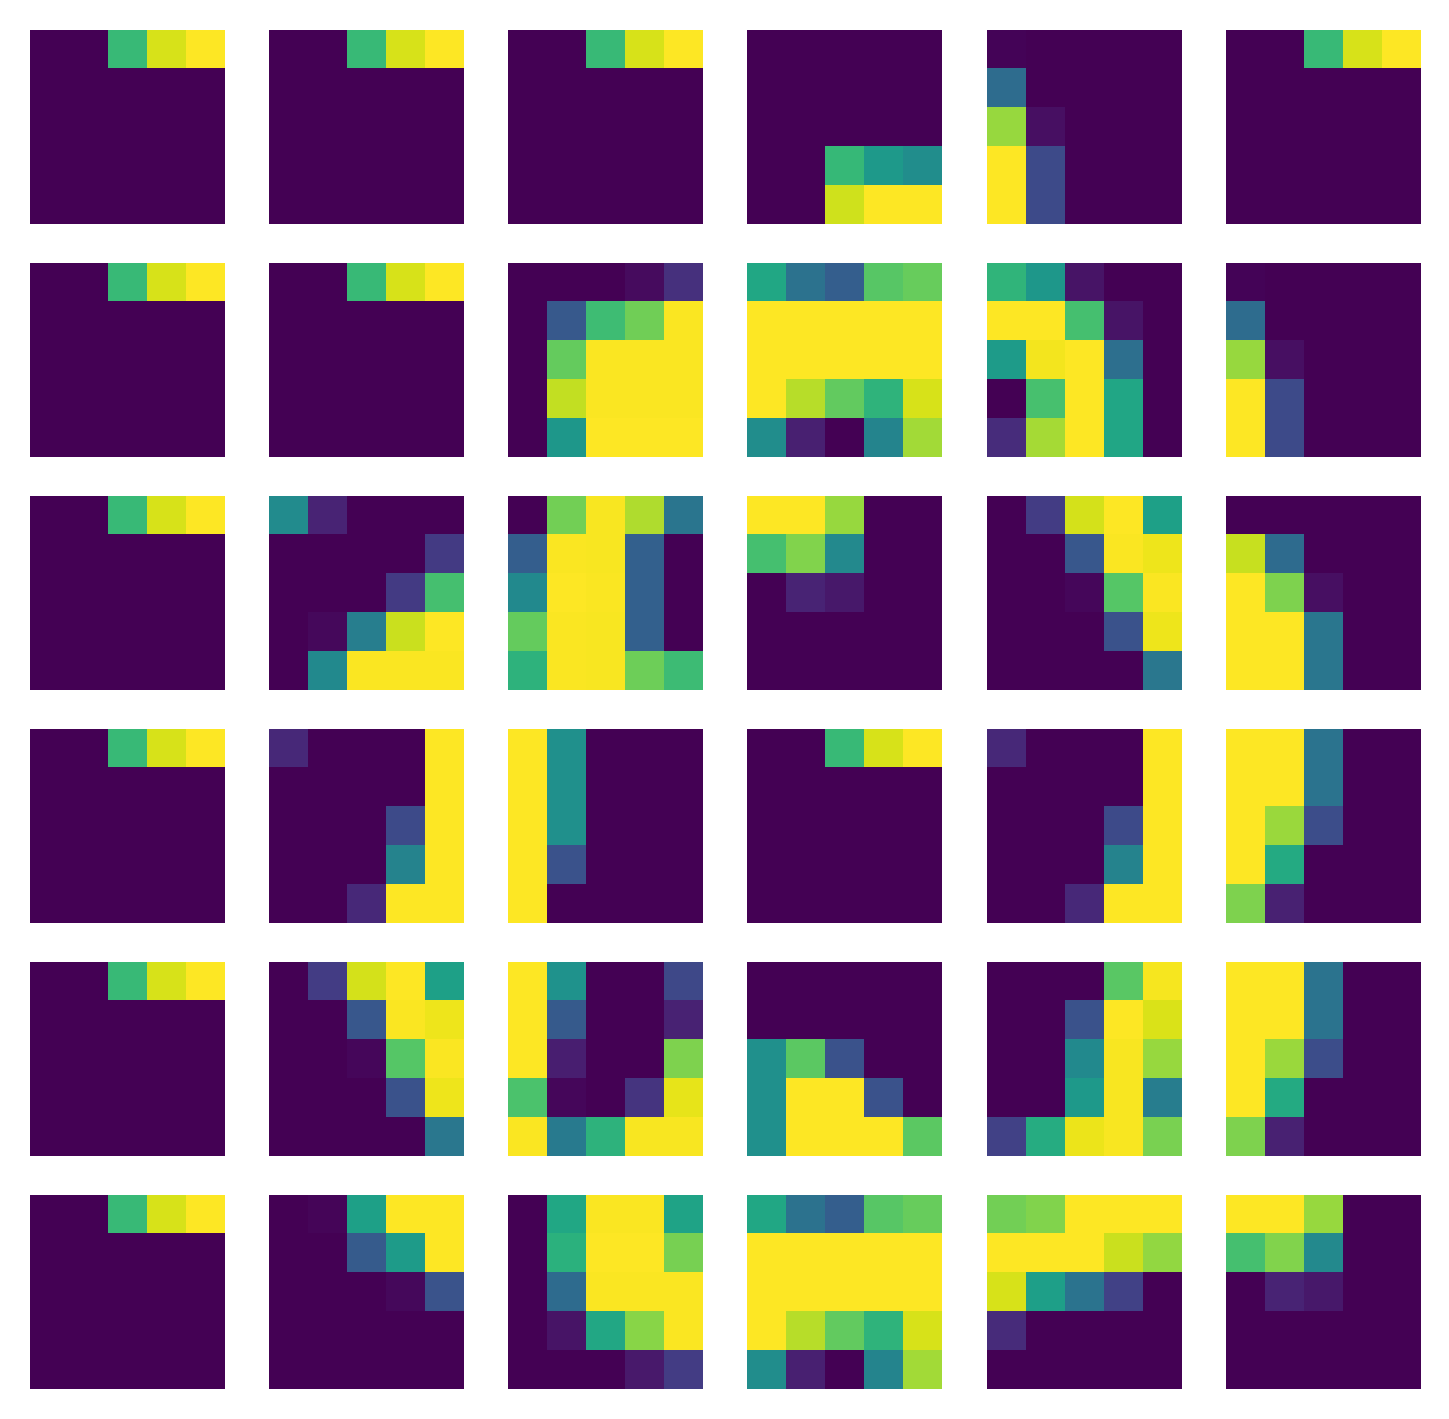
\includegraphics[width=0.9\textwidth]{CIM/mnist-16-0-cmp-rm1-ci-max-1.png}\end{minipage} &
    \begin{minipage}[t]{0.18\columnwidth}\centering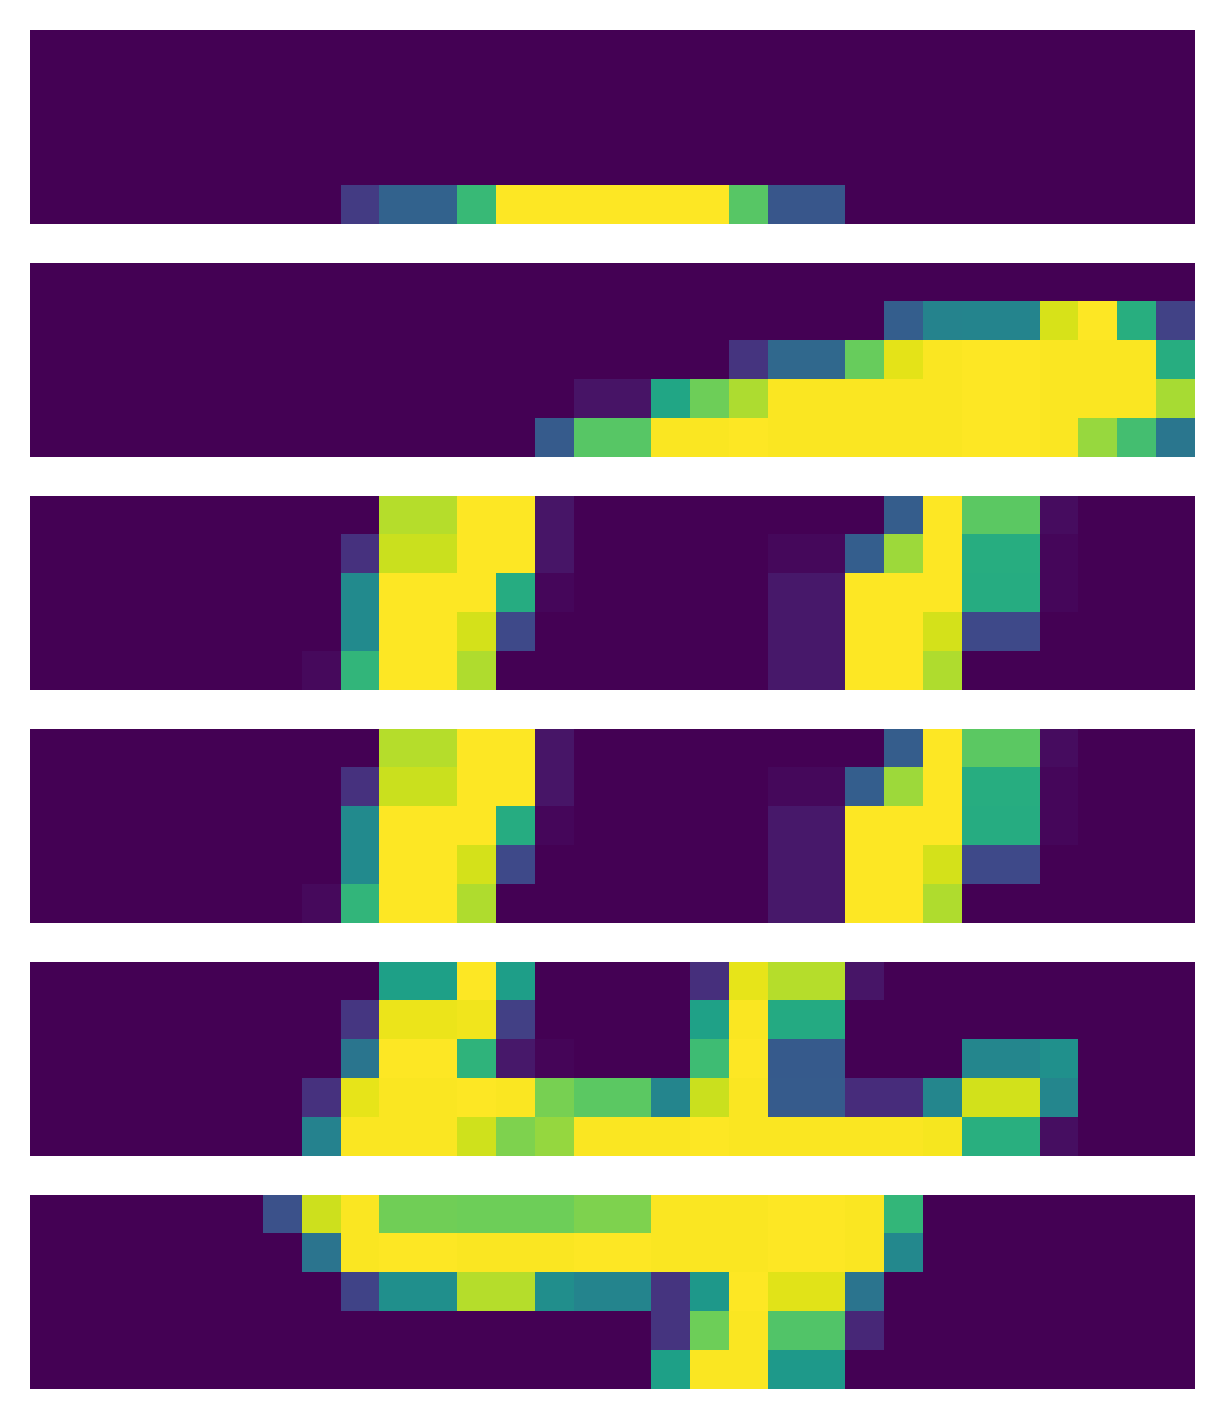
\includegraphics[width=0.9\textwidth]{CIM/mnist-16-0-cmp-rm2-ci-max-1.png}\end{minipage} &
    \begin{minipage}[t]{0.18\columnwidth}\centering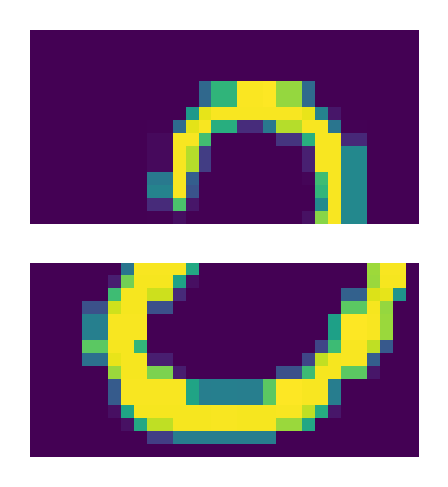
\includegraphics[width=0.9\textwidth]{CIM/mnist-16-0-cmp-rm3-ci-max-1.png}\end{minipage} &
    \begin{minipage}[t]{0.18\columnwidth}\centering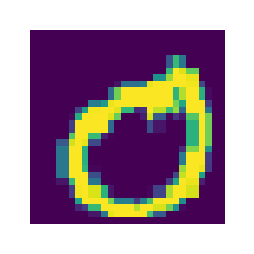
\includegraphics[width=0.9\textwidth]{CIM/mnist-16-0-cmp-rm4-ci-max-1.png}\end{minipage} 
    \\ \hline
    \end{tabular}
    \caption{特徵圖對應法示意圖\cite{YangCNNInterpretable}}
    \label{tab:CIM_RMCI_example}
\end{table}

第二個方法為全連接層權重對應法,
是透過將全連接層的輸入$x$和全連接層的權重$w$的乘積視為$RM$
並且對應之$FM$為最後一個Block的$FM$,透過此$FM$找到$CI$
將全連接層轉成可以理解的資訊。

\section{文獻回顧}

本章節將向讀者介紹可解釋性人工智慧,並回顧可解釋性人中智慧的發展歷程和分類,
協助讀者可以更了解可解釋性人工智慧的現狀與研究方向,


\subsection{可解釋性人工智慧的演進分類*}


介紹可解釋性人工智慧的歷程,分類,各分類著名的論文的簡介

可解釋性人工智慧(Explainable Artificial Intelligence, XAI)的研究最早可以追蹤到1991年的專家系統時代 W Swartout, C Paris 等人便發覺在金融、醫療,軍事等重要領域中進行的決策中往往需要一個足以支撐結論的合理解釋,
便從此開始對XAI進行研究 \cite{87686}。

XAI從一開始的小眾領域在近些年開始蓬勃發展成活躍的研究領域,
甚至每年都會有各式各樣的 Review Paper 被發表\cite{A2023100230} \cite{10188681},
論其原因應該歸功於近年來人工智慧已被各行各業所應用於分類、物件偵測、資料分析等任務,
隨著人工智慧的普及,在重要領域中XAI的地位和重要性也日益上升。

根據 \cite{Nielsen_2022} 和 \cite{LONGO2024102301} 的研究,
我們將可解釋性人工智慧的研究分為 Ante-hoc 和 Post-hoc 兩大類,
然而這兩類方法均有各自的優缺點,
值得注意的是,在\cite{LONGO2024102301}有介紹到最近有些研究展現出具有解決這兩類缺點的潛力,
但其解釋性仍須更進一步的研究,因此我們將其視為不同於前兩類的第三大類。
以下讓我們介紹這些類別的特性與較為著名的研究。

\subsection{對於 Ante-hoc explainable 模型之研究}
Ante-hoc explainable 模型(\cite{Nielsen_2022}稱為 Interently Interpretable Models),
不同於 Black Box 模型,在模型設計時就會考量可解釋性的需求,
使得模型本身便具備產生解釋性的能力,
其最終目標便是產生一個既準確又可以讓人理解決策過程的深度學習模型。

這類模型最著名的便是機器學習中的Decision Tree(DT)\cite{rokach2016decision},
DT透過一系列的規則去不斷進行抉擇並且可以很容易地被可視化,
使得人們可以容易理解DT的決策邏輯,
並且也經常被用在金融等常運用表格去表示資料的領域\cite{grinsztajn2022tree}。
除此之外也有:
一系列由DT衍伸出來的模型,例如NGE、ANFIS、、FALCON、FMMC,HRCNN, SIMTree;
由 CNN 為基礎發展出來的模型, 例如基於多層自我映射圖之可視覺化深度學習模型;
等等其他模型

然而這類模型存在一個問題便是必須再訓練模型前找出有效的特徵提取方法,
模型的可解釋性與準確度都會因為


其他模型
缺點: 需要人工整理規則或是建立有效的特徵提取方法


\subsubsection{基於多層自我映射圖之可視覺化深度學習模型}

\subsection{對於 Post-hoc 可解釋性模型之研究}
\subsubsection{Local Interpretable Model-agnostic Explanations(LIME)} 
\subsubsection{Shapley Additive Explanations(SHAP)}

\subsection{近年可解釋性模型趨勢之研究}
\subsubsection{Tabnet: Attentive interpretable tabular learning}
\subsubsection{Building more explainable artificial intelligence with argumentation}
XAI的新趨勢使用論證的方式來解釋,特別是計算論證有助於理解理性決策的所有步驟以及在不確定性下進行推理。 \cite{LONGO2024102301}



\end{document}